% Name: Torus
% Description: A torus as a surface of revolution, a circle of radius 1 swept round a circle of radius 2, shaded by height.
% Tags: torus, surface of revolution, topology, pgfplots

\usepackage{pgfplots}
\pgfplotsset{compat=1.18}

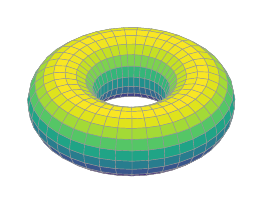
\begin{tikzpicture}
  \begin{axis}[hide axis, view={25}{35}, width=10cm, height=7cm, colormap/viridis, z buffer=sort, unit vector ratio=1 1 1]
    % ((2 + cos v) cos u, (2 + cos v) sin u, sin v)
    \addplot3[surf, faceted color=black!40, line width=0.15pt, domain=0:360, y domain=0:360, samples=40, samples y=20]
      ({(2 + cos(y))*cos(x)}, {(2 + cos(y))*sin(x)}, {sin(y)});
  \end{axis}
\end{tikzpicture}
